% 图 1.3 —— 手工重建（三圆，阴影 = 三圆交集）
%
% 做法同 1.1 / 1.2 / 2.1：看图定「是什么」，算法只在圈定区域内量「是多少」。
%
%   三个圆    实测 r = 92.4~92.7（取 92.6），圆心见下
%   阴影 = **A∩B∩C** —— 用墨迹密度验证过：
%            三圆交集处 0.30（有斜线），A/B/C 单区都是 0.00，
%            圆外 0.19 只是圆的弧穿过取样窗，不是阴影
%   阴影线    45.8°，间距 9.3，线宽 3.0
%   圆周      实测 A 4.4 / B、C 4.0
\documentclass[12pt]{standalone}
\usepackage{fontspec}
\setsansfont{Arial}
\newfontfamily\mfallback{DejaVu Sans}
\usepackage{tikz}
\usetikzlibrary{patterns}

% 阴影线：45.8°，垂直间距 9.3 → 平铺边长 9.3*sqrt(2)=13.152
% ⚠ 本图的角度不是正好 45°，平铺方块边长仍按 间距*sqrt(2) 取（斜向 ±45 时成立；
%   45.8° 与 45° 差 0.8°，对间距的影响 <0.02%，可忽略）
\pgfdeclarepatternformonly{hatch458}
  {\pgfqpoint{-13.152pt}{-13.152pt}}
  {\pgfqpoint{13.152pt}{13.152pt}}
  {\pgfqpoint{13.152pt}{13.152pt}}
  {\pgfsetlinewidth{3.0pt}\pgfsetstrokecolor{black}%
   \pgfpathmoveto{\pgfqpoint{0pt}{0pt}}%
   \pgfpathlineto{\pgfqpoint{13.152pt}{13.152pt}}%
   \pgfusepath{stroke}}

\def\rC{92.6}
\begin{document}
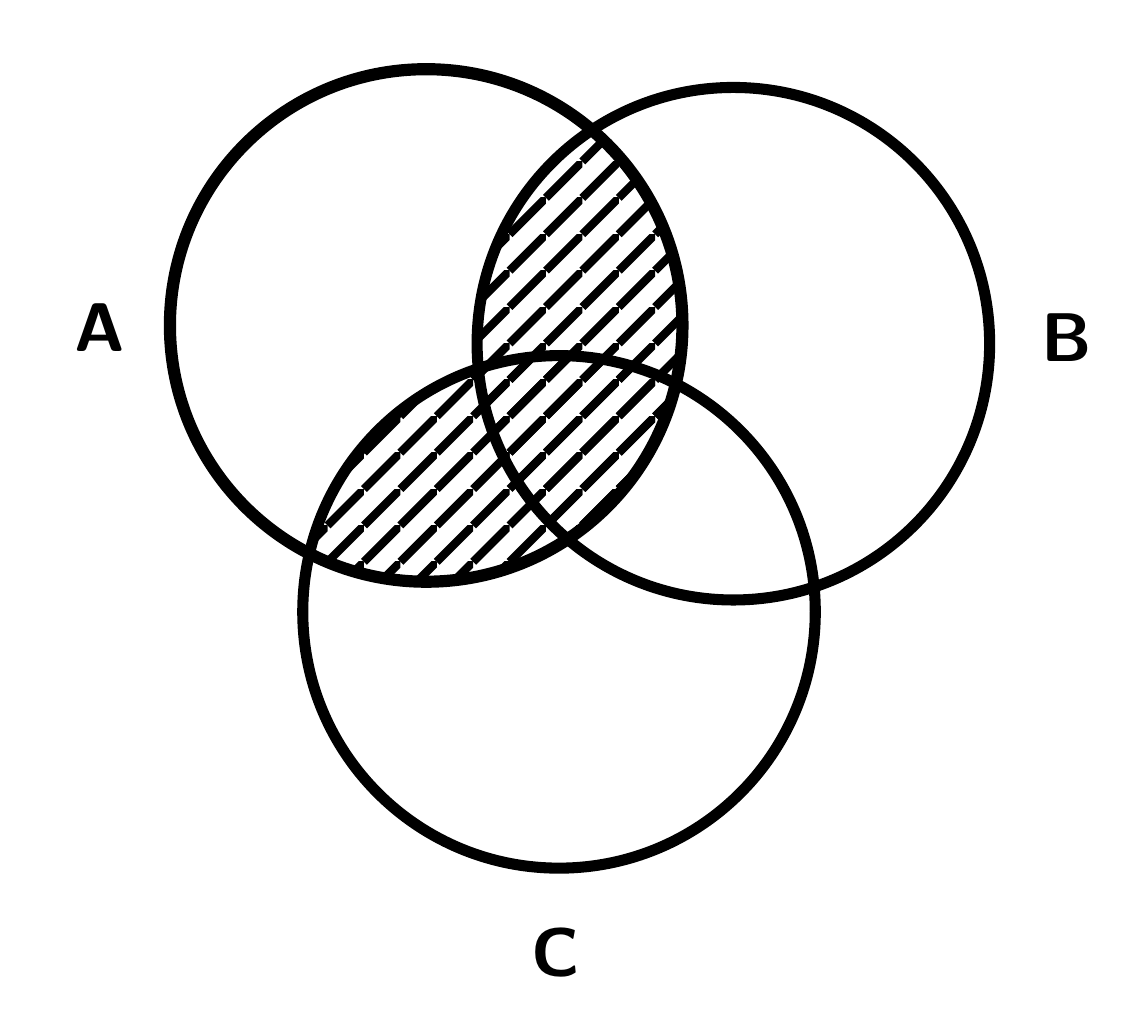
\begin{tikzpicture}[x=1pt, y=-1pt]
  \coordinate (A) at (144.0,107.6);
  \coordinate (B) at (255.0,114.2);
  \coordinate (C) at (192.0,211.1);

  % ── 阴影 = A ∩ (B∪C) ──
  % ⚠ 不是三圆交集 A∩B∩C —— 那样画会漏掉 A∩C 那一块（少了约 12% 的墨）。
  %   用墨迹密度逐点验证过：A∩B（不在 C）处有阴影、(105,180) 这种 A∩C 处也有，
  %   而 B∩C（不在 A）处没有 ⇒ 区域是 A ∩ (B∪C)。
  \begin{scope}
    \clip (A) circle (\rC);
    \fill[pattern=hatch458] (B) circle (\rC);
    \fill[pattern=hatch458] (C) circle (\rC);
  \end{scope}

  \draw[line width=4.4pt] (A) circle (\rC);
  \draw[line width=4.0pt] (B) circle (\rC);
  \draw[line width=4.0pt] (C) circle (\rC);

  % ── 标签（实测框中心 + 墨迹偏移）──
  \node[anchor=center,inner sep=1.5pt,fill=white,font=\fontsize{29.6}{37.0}\selectfont] at (26.2,108.5) {\textsf{\textbf{\textit{A}}}};
  \node[anchor=center,inner sep=1.5pt,fill=white,font=\fontsize{30.2}{37.8}\selectfont] at (375.3,112.0) {\textsf{\textbf{\textit{B}}}};
  \node[anchor=center,inner sep=1.5pt,fill=white,font=\fontsize{33.7}{42.1}\selectfont] at (190.8,334.3) {\textsf{\textbf{\textit{C}}}};

  \path[use as bounding box] (0,0) rectangle (392,354);
\end{tikzpicture}
\end{document}
